%% ============================================================
%%  NewsChecker DApp — Documentation Académique Professionnelle
%%  Compatible XeLaTeX (Tectonic)
%% ============================================================
\documentclass[12pt,a4paper]{article}

%% ── Encodage XeLaTeX ─────────────────────────────────────────
\usepackage{fontspec}
\usepackage{polyglossia}
\setmainlanguage{french}

%% ── Mise en page ─────────────────────────────────────────────
\usepackage[top=2.5cm, bottom=2.5cm, left=2.8cm, right=2.8cm]{geometry}
\usepackage{fancyhdr}
\usepackage{titlesec}
\usepackage{parskip}
\usepackage{setspace}
\setstretch{1.15}

%% ── Polices ──────────────────────────────────────────────────
\usepackage{microtype}

%% ── Couleurs ─────────────────────────────────────────────────
\usepackage[dvipsnames,svgnames,x11names]{xcolor}
\definecolor{primary}{HTML}{6366F1}
\definecolor{accent}{HTML}{06B6D4}
\definecolor{success}{HTML}{10B981}
\definecolor{danger}{HTML}{EF4444}
\definecolor{warning}{HTML}{F59E0B}
\definecolor{darkbg}{HTML}{0F172A}
\definecolor{cardbg}{HTML}{1E293B}
\definecolor{lightgray}{HTML}{F1F5F9}
\definecolor{codebg}{HTML}{1E293B}
\definecolor{codefg}{HTML}{E2E8F0}
\definecolor{mutedtext}{HTML}{94A3B8}

%% ── Liens ────────────────────────────────────────────────────
\usepackage[colorlinks=true,
            linkcolor=primary,
            urlcolor=accent,
            citecolor=success,
            pdftitle={NewsChecker DApp Documentation},
            pdfauthor={Equipe NewsChecker}]{hyperref}

%% ── Maths ────────────────────────────────────────────────────
\usepackage{amsmath}
\usepackage{amssymb}

%% ── Graphiques ───────────────────────────────────────────────
\usepackage{graphicx}
\usepackage{float}
\usepackage{caption}
\usepackage{subcaption}
\captionsetup{font=small, labelfont={bf,color=primary}, textfont=it}

%% ── TikZ ─────────────────────────────────────────────────────
\usepackage{tikz}
\usepackage{pgfplots}
\pgfplotsset{compat=1.18}
\usetikzlibrary{
  arrows.meta, positioning, shapes.geometric,
  fit, calc, backgrounds, decorations.pathreplacing,
  decorations.markings, matrix
}

%% ── Tableaux ─────────────────────────────────────────────────
\usepackage{booktabs}
\usepackage{longtable}
\usepackage{array}
\usepackage{multirow}
\usepackage{colortbl}
\newcolumntype{L}[1]{>{\raggedright\arraybackslash}p{#1}}
\newcolumntype{C}[1]{>{\centering\arraybackslash}p{#1}}

%% ── Code ─────────────────────────────────────────────────────
\usepackage{listings}
\lstset{
  backgroundcolor=\color{codebg},
  basicstyle=\ttfamily\scriptsize\color{codefg},
  keywordstyle=\color{primary}\bfseries,
  commentstyle=\color{mutedtext}\itshape,
  stringstyle=\color{success},
  numberstyle=\tiny\color{mutedtext},
  numbers=left,
  stepnumber=1,
  numbersep=8pt,
  breaklines=true,
  frame=single,
  framerule=0.5pt,
  rulecolor=\color{primary!40},
  tabsize=2,
  showstringspaces=false,
  captionpos=b,
  xleftmargin=1.5em,
}
\lstdefinelanguage{SmartPy}{
  morekeywords={sp,module,class,def,self,assert,if,else,for,in,True,False,
    and,or,not,import,return,with,while},
  sensitive=true,
  morecomment=[l]{\#},
  morestring=[b]",
  morestring=[b]'
}
\lstdefinelanguage{JSX}{
  morekeywords={import,export,from,const,let,var,function,return,async,
    await,if,else,true,false,null,new,class,extends,default},
  sensitive=true,
  morecomment=[l]{//},
  morecomment=[s]{/*}{*/},
  morestring=[b]",
  morestring=[b]'
}

%% ── Boîtes ───────────────────────────────────────────────────
\usepackage{tcolorbox}
\tcbuselibrary{skins, breakable}

\newenvironment{infobox}[1][Info]{%
  \begin{tcolorbox}[
    enhanced, breakable,
    colback=accent!8, colframe=accent!70, coltitle=white,
    title=\textbf{#1}, fonttitle=\small,
    arc=4pt, boxrule=0.8pt,
    left=6pt, right=6pt, top=5pt, bottom=5pt
  ]
}{\end{tcolorbox}}

\newenvironment{warnbox}[1][Attention]{%
  \begin{tcolorbox}[
    enhanced, breakable,
    colback=warning!8, colframe=warning!70, coltitle=white,
    title=\textbf{#1}, fonttitle=\small,
    arc=4pt, boxrule=0.8pt,
    left=6pt, right=6pt, top=5pt, bottom=5pt
  ]
}{\end{tcolorbox}}

\newenvironment{successbox}[1][Résultat]{%
  \begin{tcolorbox}[
    enhanced, breakable,
    colback=success!8, colframe=success!70, coltitle=white,
    title=\textbf{#1}, fonttitle=\small,
    arc=4pt, boxrule=0.8pt,
    left=6pt, right=6pt, top=5pt, bottom=5pt
  ]
}{\end{tcolorbox}}

\newenvironment{dangerbox}[1][Important]{%
  \begin{tcolorbox}[
    enhanced, breakable,
    colback=danger!8, colframe=danger!70, coltitle=white,
    title=\textbf{#1}, fonttitle=\small,
    arc=4pt, boxrule=0.8pt,
    left=6pt, right=6pt, top=5pt, bottom=5pt
  ]
}{\end{tcolorbox}}

%% ── En-tête/Pied de page ─────────────────────────────────────
\pagestyle{fancy}
\fancyhf{}
\fancyhead[L]{\small\color{mutedtext}\textbf{NewsChecker DApp}}
\fancyhead[R]{\small\color{mutedtext}Documentation Technique}
\fancyfoot[C]{\small\color{mutedtext}\thepage}
\fancyfoot[R]{\small\color{mutedtext}Tezos Ghostnet}
\renewcommand{\headrulewidth}{0.4pt}
\renewcommand{\footrulewidth}{0.4pt}

%% ── Titres ───────────────────────────────────────────────────
\titleformat{\section}
  {\Large\bfseries\color{darkbg}}
  {\colorbox{primary}{\color{white}\thesection}}{0.8em}{}
  [\vspace{-0.2em}\color{primary}\hrulefill]

\titleformat{\subsection}
  {\large\bfseries\color{darkbg}}
  {\color{primary}\thesubsection}{0.7em}{}

\titleformat{\subsubsection}
  {\normalsize\bfseries\color{darkbg}}
  {\color{accent}\thesubsubsection}{0.6em}{}

%% ── Commandes utiles ─────────────────────────────────────────
\newcommand{\tezos}{\textcolor{primary}{\textbf{Tezos}}}
\newcommand{\smartpy}{\textcolor{accent}{\textbf{SmartPy}}}
\newcommand{\reactjs}{\textcolor{success}{\textbf{React}}}
\newcommand{\taquito}{\textcolor{warning}{\textbf{Taquito}}}
\newcommand{\beacon}{\textcolor{primary}{\textbf{Beacon}}}
\newcommand{\entrypoint}[1]{\textcolor{primary}{\texttt{\textbf{#1}}}}
\newcommand{\status}[2]{\textcolor{#1}{\textbf{\texttt{#2}}}}

%% ============================================================
\begin{document}

%% ════════════════════════════════════════════════════════════
%%  PAGE DE TITRE  (design simple et professionnel)
%% ════════════════════════════════════════════════════════════
\begin{titlepage}
\newgeometry{top=0pt,bottom=0pt,left=0pt,right=0pt}

%% Filet coloré haut
\begin{tikzpicture}[remember picture,overlay]
  \fill[primary] (current page.north west) rectangle ++(21cm,-0.9cm);
\end{tikzpicture}

\vspace*{3.5cm}
\begin{center}

%% ── Titre ────────────────────────────────────────────────────
{\fontsize{48}{56}\bfseries\color{darkbg} NewsChecker}

\vspace{0.4cm}
{\Large\color{primary}\itshape
  Application Décentralisée de Vérification des Informations}

\vspace{0.5cm}
\textcolor{primary!50}{\rule{11cm}{1.2pt}}

\vspace{0.5cm}
{\normalsize\color{darkbg!60}
  Contrat Intelligent \textbf{SmartPy} sur \textbf{Tezos Ghostnet}
  \enspace$\cdot$\enspace
  Interface \textbf{React\,19} + \textbf{Taquito\,24}}

\vspace{3.5cm}

%% ── Auteurs ──────────────────────────────────────────────────
{\normalsize\color{darkbg!50}\scshape Réalisé par}

\vspace{0.9cm}

{\large\color{darkbg}
\begin{tabular}{c}
  Maram \textbf{Arfaoui}\\[0.7em]
  Abderrazzak \textbf{El Bourkadi}\\[0.7em]
  Ayoub \textbf{Et-Toubi}\\[0.7em]
  Asmaa \textbf{Assaid}\\[0.7em]
  Mohamed \textbf{Cheikh}\\
\end{tabular}}

\vspace{3.2cm}
\textcolor{primary!50}{\rule{11cm}{0.6pt}}
\vspace{0.6cm}

%% ── Informations projet ──────────────────────────────────────
{\small\color{darkbg!55}
  \begin{tabular}{r@{\hspace{0.5em}:\hspace{0.7em}}l}
    Réseau  & Tezos Ghostnet (Testnet) \\[0.25em]
    Contrat & \texttt{KT1H49BAbxYfBReehN4dShGpm6jVWapXPgeq} \\[0.25em]
    Version & 1.0.0\quad$\cdot$\quad Mars 2026 \\
  \end{tabular}}

\end{center}

%% Filet coloré bas
\begin{tikzpicture}[remember picture,overlay]
  \fill[primary] (current page.south west) rectangle ++(21cm,0.9cm);
\end{tikzpicture}

\restoregeometry
\end{titlepage}

%% ════════════════════════════════════════════════════════════
%%  RÉSUMÉ
%% ════════════════════════════════════════════════════════════
\newpage
\begin{abstract}
\noindent
\textbf{NewsChecker} est une application décentralisée (DApp) déployée sur la blockchain \tezos{} qui permet la vérification collective et transparente d'articles de presse. Le système s'appuie sur un contrat intelligent écrit en \smartpy{}, combinant un mécanisme de mise en jeu (\emph{staking}) économique, un système de réputation progressif, et un vote pondéré résistant aux attaques Sybil.

Les membres s'inscrivent en verrouillant une mise minimale en Tez, soumettent des articles à vérifier, et votent sur leur authenticité. Le poids de chaque vote est nul jusqu'à ce qu'un membre atteigne le seuil de réputation (5 points, soit le statut \emph{Voter Confirmé}), puis devient égal à sa réputation. La finalisation d'un vote suit deux modes : \textbf{Mode A} (quorum atteint + délai minimum écoulé) ou \textbf{Mode B} (deadline dépassée avec au moins un vote). Les votants corrects voient leur réputation augmenter de $+2$, les votants incorrects subissent une pénalité de $-3$.

L'interface web \reactjs{}, connectée via la bibliothèque \taquito{} et le protocole \beacon{}, offre quatre panneaux fonctionnels : Dashboard, News, Member et Admin. Un mode Démo permet l'exploration complète sans portefeuille réel.
\end{abstract}

\newpage
\tableofcontents
\newpage

%% ════════════════════════════════════════════════════════════
\section{Introduction}
%% ════════════════════════════════════════════════════════════

\subsection{Problématique}

La prolifération de fausses informations sur internet constitue l'un des défis majeurs de notre époque numérique. Les plateformes centralisées de fact-checking présentent des vulnérabilités inhérentes : biais éditoriaux, point de défaillance unique, manque de transparence dans les processus de décision, et risque de censure arbitraire.

\begin{dangerbox}[Problèmes des systèmes centralisés]
\begin{itemize}
  \item \textbf{Point de confiance unique :} L'autorité centrale peut être corrompue ou compromise
  \item \textbf{Attaques Sybil :} Un acteur malveillant peut créer de multiples comptes pour manipuler les votes
  \item \textbf{Absence de traçabilité :} Les décisions de modération sont opaques et non vérifiables
  \item \textbf{Résistance à la censure :} Aucune garantie contre la suppression d'informations légitimes
\end{itemize}
\end{dangerbox}

\subsection{Objectifs du projet}

NewsChecker propose une alternative décentralisée reposant sur les propriétés fondamentales de la blockchain \tezos{} :

\begin{successbox}[Objectifs principaux]
\begin{enumerate}
  \item \textbf{Décentralisation :} Aucune autorité centrale --- le contrat intelligent est la loi
  \item \textbf{Transparence :} Toutes les données (votes, réputations, stakes) sont publiques sur la chaîne
  \item \textbf{Résistance Sybil :} Le mécanisme de réputation progressive neutralise les comptes fantômes
  \item \textbf{Incitation économique :} Le staking engage financièrement les participants à voter honnêtement
  \item \textbf{Gouvernance évolutive :} L'administrateur peut ajuster les paramètres sans redéploiement
\end{enumerate}
\end{successbox}

\subsection{Contributions principales}

\begin{itemize}
  \item Conception d'un contrat intelligent \smartpy{} avec 7 points d'entrée (\emph{entrypoints})
  \item Implémentation d'un système de réputation bi-état (Probatoire / Confirmé)
  \item Double mécanisme de finalisation pour gérer les cas de faible participation
  \item Interface DApp \reactjs{} complète avec mode Démo intégré
  \item Suite de tests automatisés (8 scénarios couvrant les cas nominaux et adversariaux)
\end{itemize}

%% ════════════════════════════════════════════════════════════
\section{Architecture du Système}
%% ════════════════════════════════════════════════════════════

\subsection{Vue d'ensemble technologique}

\begin{figure}[H]
\centering
\begin{tikzpicture}[
  node distance=0.9cm and 1.6cm,
  box/.style={draw, rounded corners=6pt, minimum width=2.6cm,
              minimum height=1.0cm, align=center, font=\small\bfseries,
              line width=1.2pt},
  arrow/.style={-{Stealth[length=6pt]}, line width=1.5pt}
]

\node[box, fill=primary!20, draw=primary] (user)
  {\textcolor{primary}{Utilisateur}\\{\scriptsize Temple / Kukai}};

\node[box, fill=warning!20, draw=warning, right=of user] (beacon)
  {\textcolor{warning}{Beacon}\\{\scriptsize Wallet SDK}};

\node[box, fill=success!20, draw=success, right=of beacon] (react)
  {\textcolor{success}{React DApp}\\{\scriptsize Vite 8}};

\node[box, fill=accent!20, draw=accent, below=of react] (taquito)
  {\textcolor{accent}{Taquito}\\{\scriptsize Tezos Toolkit}};

\node[box, fill=primary!15, draw=primary!70, left=of taquito] (node)
  {\textcolor{primary}{Tezos Node}\\{\scriptsize Ghostnet}};

\node[box, fill=danger!20, draw=danger, left=of node] (contract)
  {\textcolor{danger}{NewsChecker}\\{\scriptsize KT1...}};

\draw[arrow, primary]  (user)    -- node[above, font=\tiny]{sign}    (beacon);
\draw[arrow, warning]  (beacon)  -- node[above, font=\tiny]{auth}    (react);
\draw[arrow, success]  (react)   -- node[right, font=\tiny]{calls}   (taquito);
\draw[arrow, accent]   (taquito) -- node[above, font=\tiny]{RPC}     (node);
\draw[arrow, primary!70] (node)  -- node[above, font=\tiny]{Michelson} (contract);

\draw[arrow, danger, dashed] (contract) to[bend left=25]
  node[below, font=\tiny]{storage} (taquito);
\draw[arrow, accent, dashed]  (taquito) to[bend right=15]
  node[right, font=\tiny]{state} (react);

\end{tikzpicture}
\caption{Architecture globale du système NewsChecker}
\label{fig:arch}
\end{figure}

\subsection{Stack technique}

\begin{table}[H]
\centering
\renewcommand{\arraystretch}{1.4}
\begin{tabular}{L{3cm} L{3.5cm} L{6cm}}
\toprule
\rowcolor{primary!15}
\textbf{Couche} & \textbf{Technologie} & \textbf{Rôle} \\
\midrule
Smart Contract    & SmartPy 0.20     & Logique métier on-chain (Python $\to$ Michelson) \\
\rowcolor{lightgray}
Réseau            & Tezos Ghostnet   & Blockchain Layer-1, consensus proof-of-stake \\
RPC Client        & Taquito 20       & Communication JavaScript $\leftrightarrow$ nœud Tezos \\
\rowcolor{lightgray}
Wallet            & Beacon SDK 4     & Protocole de connexion portefeuille universel \\
Frontend          & React 19 + Vite 8 & Interface utilisateur réactive \\
\rowcolor{lightgray}
Styles            & Tailwind CSS 4   & Design system utilitaire \\
Icônes            & Lucide React     & Bibliothèque d'icônes SVG \\
\rowcolor{lightgray}
Notifications     & React Hot Toast  & Retours utilisateur en temps réel \\
\bottomrule
\end{tabular}
\caption{Stack technique complet du projet}
\end{table}

%% ════════════════════════════════════════════════════════════
\section{Smart Contract NewsChecker}
%% ════════════════════════════════════════════════════════════

\subsection{Vue d'ensemble}

Le contrat \texttt{NewsChecker} est écrit en \smartpy{} et orchestre l'intégralité de la logique de vérification des nouvelles. Il gère les membres, les articles, les votes, et les réputations de manière entièrement autonome et transparente.

\begin{infobox}[Paramètres d'initialisation]
\begin{tabular}{L{3.5cm} L{2.5cm} L{6cm}}
\textbf{Paramètre} & \textbf{Valeur démo} & \textbf{Description} \\
\midrule
\texttt{admin}          & \texttt{tz1Admin...} & Adresse administrateur \\
\texttt{min\_stake}     & 1\,000\,000 µtez     & Mise minimale (1 tez) \\
\texttt{quorum}         & 3                    & Votes requis (Mode A) \\
\texttt{rep\_threshold} & 5                    & Seuil réputation pondérée \\
\texttt{vote\_delay}    & 3\,600 s             & Délai min. avant finalisation (1h) \\
\texttt{vote\_duration} & 86\,400 s            & Durée maximale du vote (24h) \\
\end{tabular}
\end{infobox}

\subsection{Structures de données}

\subsubsection{Storage du contrat}

\begin{table}[H]
\centering
\renewcommand{\arraystretch}{1.4}
\begin{tabular}{L{3.2cm} L{4.2cm} L{5cm}}
\toprule
\rowcolor{primary!15}
\textbf{Champ} & \textbf{Type SmartPy} & \textbf{Description} \\
\midrule
\texttt{admin}          & \texttt{sp.address}            & Adresse administrateur \\
\rowcolor{lightgray}
\texttt{min\_stake}     & \texttt{sp.mutez}              & Mise minimale requise \\
\texttt{quorum}         & \texttt{sp.nat}                & Nb. votes pour Mode A \\
\rowcolor{lightgray}
\texttt{rep\_threshold} & \texttt{sp.nat}                & Seuil réputation pondérée \\
\texttt{vote\_delay}    & \texttt{sp.int}                & Délai min (secondes) \\
\rowcolor{lightgray}
\texttt{vote\_duration} & \texttt{sp.int}                & Durée max (secondes) \\
\texttt{next\_news\_id} & \texttt{sp.nat}                & Compteur auto-incrémenté \\
\rowcolor{lightgray}
\texttt{members}        & \texttt{big\_map[addr, Member]} & Membres inscrits \\
\texttt{news}           & \texttt{big\_map[nat, News]}   & Articles soumis \\
\rowcolor{lightgray}
\texttt{votes}          & \texttt{big\_map[(nat,addr), bool]} & Votes individuels \\
\texttt{voters}         & \texttt{big\_map[nat, list[addr]]}  & Votants par article \\
\bottomrule
\end{tabular}
\caption{Structure du storage du contrat NewsChecker}
\end{table}

\subsubsection{Enregistrements SmartPy}

\begin{lstlisting}[language=SmartPy, caption={Structure Member et NewsItem}]
# Enregistrement d'un membre
sp.record(
    reputation = sp.nat,    # Points de reputation (debut: 1)
    staked     = sp.mutez,  # Montant verrouille en Tez
    active     = sp.bool    # Statut actif/inactif
)

# Enregistrement d'un article
sp.record(
    author      = sp.address,    # Soumetteur
    title       = sp.string,     # Titre
    url         = sp.string,     # URL source
    status      = sp.nat,        # 1=Vote, 2=Reel, 3=Fake
    votes_real  = sp.nat,        # Somme ponderee REEL
    votes_fake  = sp.nat,        # Somme ponderee FAKE
    count_real  = sp.nat,        # Votes bruts REEL
    count_fake  = sp.nat,        # Votes bruts FAKE
    submit_time = sp.timestamp   # Horodatage soumission
)
\end{lstlisting}

\subsection{Les 7 points d'entrée}

\subsubsection{\entrypoint{register} — Inscription}

\begin{lstlisting}[language=SmartPy, caption={Entrypoint register}]
@sp.entrypoint
def register(self):
    assert not self.data.members.contains(sp.sender), "ALREADY_REGISTERED"
    assert sp.amount >= self.data.min_stake, "INSUFFICIENT_STAKE"
    self.data.members[sp.sender] = sp.record(
        reputation = sp.nat(1),   # Mode probatoire (poids=0)
        staked     = sp.amount,
        active     = True
    )
\end{lstlisting}

\begin{infobox}[Logique register]
L'inscription requiert un paiement on-chain d'au moins \texttt{min\_stake} mutez. La réputation initiale de 1 place le membre en mode \textbf{Probatoire} --- ses votes ne comptent pas dans le total pondéré tant qu'il n'atteint pas le seuil de 5.
\end{infobox}

\subsubsection{\entrypoint{vote} — Vote pondéré par réputation}

\begin{lstlisting}[language=SmartPy, caption={Entrypoint vote avec poids de reputation}]
@sp.entrypoint
def vote(self, news_id, opinion):
    n = self.data.news[news_id]
    assert n.status == sp.nat(1), "NOT_IN_VOTING"
    deadline = sp.add_seconds(n.submit_time, self.data.vote_duration)
    assert sp.now < deadline, "VOTING_ENDED"      # Deadline
    m = self.data.members[sp.sender]
    assert m.staked >= self.data.min_stake, "STAKE_TOO_LOW"
    key = (news_id, sp.sender)
    assert not self.data.votes.contains(key), "ALREADY_VOTED"
    # Poids: 0 si probatoire, reputation si confirme
    w = sp.nat(0)
    if m.reputation >= self.data.rep_threshold:
        w = m.reputation
    # Enregistrement avec poids
    if opinion:
        # votes_real += w, count_real += 1
    else:
        # votes_fake += w, count_fake += 1
\end{lstlisting}

\subsubsection{\entrypoint{finalize} — Clôture du vote}

\begin{figure}[H]
\centering
\begin{tikzpicture}[
  node distance=1.0cm and 1.5cm,
  box/.style={draw, rounded corners=4pt, minimum width=3cm,
              minimum height=0.75cm, align=center, font=\small},
  diam/.style={draw, diamond, aspect=2.2, minimum width=3.2cm,
               minimum height=0.9cm, align=center, font=\small},
  arr/.style={-{Stealth}, line width=1.2pt}
]

\node[box, fill=warning!20, draw=warning] (start) {\textbf{finalize(news\_id)}};
\node[diam, fill=primary!10, draw=primary, below=of start] (d1)
  {Quorum atteint?};
\node[diam, fill=primary!10, draw=primary, right=2.5cm of d1] (d2)
  {Délai min écoulé?};
\node[diam, fill=accent!10, draw=accent, below=1.8cm of d1] (d3)
  {Deadline passée?};
\node[box, fill=success!20, draw=success, below=1.5cm of d2] (modeA)
  {\textbf{Mode A} : Quorum+Délai};
\node[box, fill=accent!20, draw=accent, below=1.5cm of d3] (modeB)
  {\textbf{Mode B} : Timeout};
\node[box, fill=danger!20, draw=danger, right=1.8cm of d3] (fail)
  {\texttt{CANNOT\_FINALIZE\_YET}};
\node[box, fill=warning!20, draw=warning, below=1.8cm of modeA] (result)
  {votes\_real $>$ votes\_fake?};
\node[box, fill=success!30, draw=success, right=1.5cm of result] (real)
  {\status{success}{status = 2 (RÉEL)}};
\node[box, fill=danger!30, draw=danger, below=of result] (fake)
  {\status{danger}{status = 3 (FAKE)}};
\node[box, fill=primary!20, draw=primary, below=of fake] (rep)
  {Mise à jour réputations};

\draw[arr, primary] (start) -- (d1);
\draw[arr, success] (d1)    -- node[above,font=\tiny]{Oui} (d2);
\draw[arr, danger]  (d1)    -- node[left, font=\tiny]{Non} (d3);
\draw[arr, success] (d2)    -- node[right,font=\tiny]{Oui} (modeA);
\draw[arr, danger]  (d2) -| node[above right,font=\tiny]{Non} (fail);
\draw[arr, success] (d3)    -- node[left, font=\tiny]{Oui} (modeB);
\draw[arr, danger]  (d3)    -- node[above,font=\tiny]{Non} (fail);
\draw[arr, success] (modeA) -- (result);
\draw[arr, success] (modeB) -| (result);
\draw[arr, success] (result) -- node[above,font=\tiny]{Oui} (real);
\draw[arr, danger]  (result) -- node[left, font=\tiny]{Non} (fake);
\draw[arr, primary] (real) |- (rep);
\draw[arr, primary] (fake) -- (rep);

\end{tikzpicture}
\caption{Flowchart du processus de finalisation (deux modes)}
\label{fig:finalize}
\end{figure}

\subsubsection{\entrypoint{add\_stake}, \entrypoint{withdraw\_stake} et \entrypoint{update\_params}}

\begin{lstlisting}[language=SmartPy, caption={Gestion du stake et paramètres admin}]
@sp.entrypoint
def add_stake(self):
    m = self.data.members[sp.sender]
    self.data.members[sp.sender] = sp.record(
        reputation=m.reputation,
        staked=m.staked + sp.amount,  # Ajoute le montant envoye
        active=m.active)

@sp.entrypoint
def withdraw_stake(self, amount):
    m = self.data.members[sp.sender]
    remaining = m.staked - amount
    assert remaining >= self.data.min_stake, "BELOW_MINIMUM"
    sp.send(sp.sender, amount)  # Transfert on-chain

@sp.entrypoint
def update_params(self, new_min_stake, new_quorum, ...):
    assert sp.sender == self.data.admin, "NOT_ADMIN"
    self.data.min_stake     = new_min_stake
    self.data.quorum        = new_quorum
    # ... autres parametres
\end{lstlisting}

\subsection{Système de réputation}

\subsubsection{Machine à états}

\begin{figure}[H]
\centering
\begin{tikzpicture}[
  state/.style={draw, circle, minimum size=3cm, align=center,
                font=\small\bfseries, line width=1.5pt},
  arr/.style={-{Stealth[length=7pt]}, line width=1.8pt}
]
\node[state, fill=warning!25, draw=warning] (prob) at (0,0)
  {\textcolor{warning}{Probatoire}\\{\small rep $< 5$}\\{\footnotesize poids $= 0$}};

\node[state, fill=success!25, draw=success] (conf) at (8,0)
  {\textcolor{success}{Confirmé}\\{\small rep $\geq 5$}\\{\footnotesize poids $=$ rep}};

\draw[arr, success, bend left=25] (prob) to
  node[above, font=\scriptsize]{\textcolor{success}{+2 (vote correct)}} (conf);

\draw[arr, danger, bend left=25] (conf) to
  node[below, font=\scriptsize]{\textcolor{danger}{-3 (vote incorrect)}} (prob);

\draw[arr, success, loop above, looseness=4] (conf) to
  node[above, font=\scriptsize]{\textcolor{success}{+2}} (conf);

\draw[arr, warning, loop above, looseness=4] (prob) to
  node[above, font=\scriptsize]{\textcolor{warning}{+2}} (prob);

\draw[dashed, primary, line width=1pt] (4,-2) -- (4,2.5);
\node[above, font=\small\bfseries, text=primary] at (4,2.5){Seuil = 5};

\node[below=0.5cm of prob, font=\scriptsize\itshape, text=mutedtext]
  {Inscription initiale : rep = 1};
\end{tikzpicture}
\caption{Machine à états du système de réputation}
\label{fig:reputation}
\end{figure}

\subsubsection{Évolution de la réputation}

\begin{table}[H]
\centering
\renewcommand{\arraystretch}{1.5}
\begin{tabular}{L{4.5cm} C{3cm} C{2cm} C{3cm}}
\toprule
\rowcolor{primary!15}
\textbf{Situation} & \textbf{Rép. avant} & \textbf{Delta} & \textbf{Rép. après} \\
\midrule
Vote correct (probatoire, tour 1) & 1 & \textcolor{success}{+2} & 3 \\
\rowcolor{lightgray}
Vote correct (probatoire, tour 2) & 3 & \textcolor{success}{+2} & \textbf{5 ✓ Confirmé} \\
Vote correct (confirmé)           & 5 & \textcolor{success}{+2} & 7 \\
\rowcolor{lightgray}
Vote incorrect (confirmé)         & 7 & \textcolor{danger}{-3}  & 4 ← Probatoire \\
Vote incorrect (rep $\leq$ 4)     & 4 & \textcolor{danger}{-3 (min 1)} & 1 \\
\bottomrule
\end{tabular}
\caption{Évolution de la réputation selon les votes}
\end{table}

\subsection{Protection anti-Sybil}

\begin{warnbox}[Résistance aux attaques Sybil]
Un attaquant créant $N$ comptes en probatoire (rep = 1) ne peut pas influencer le résultat car le \textbf{poids pondéré} de chacun est 0. Seuls les membres \textbf{Confirmés} (rep $\geq 5$) ont un poids effectif.

\medskip
\textbf{Exemple (test Sybil)} : 5 attaquants (poids = 0) votent RÉEL vs 2 confirmés (poids = 5 chacun) votant FAKE :
$$\text{votes\_real} = 5 \times 0 = 0 \quad \text{vs} \quad \text{votes\_fake} = 2 \times 5 = 10$$
$$\Rightarrow \text{Résultat : \textbf{FAKE}} \quad \checkmark$$
\end{warnbox}

%% ════════════════════════════════════════════════════════════
\section{Interface DApp (React)}
%% ════════════════════════════════════════════════════════════

\subsection{Architecture des composants}

\begin{figure}[H]
\centering
\begin{tikzpicture}[
  comp/.style={draw, rounded corners=4pt, minimum width=2.8cm,
               minimum height=0.8cm, align=center, font=\small\bfseries,
               line width=1pt},
  ctx/.style={draw, dashed, rounded corners=5pt, minimum width=3.2cm,
              minimum height=0.8cm, align=center, font=\small,
              line width=1pt, draw=accent},
  arr/.style={-{Stealth}, line width=1pt, primary}
]

\node[ctx, fill=accent!10] (ctx) at (0,4.5)
  {\textcolor{accent}{\textbf{WalletContext}}\\{\tiny useWallet() hook}};

\node[comp, fill=primary!20, draw=primary] (app) at (0,3)
  {\textcolor{primary}{App.jsx}};

\node[comp, fill=warning!20, draw=warning]  (nav)    at (-5.5,1.2) {\textcolor{warning}{Navbar.jsx}};
\node[comp, fill=success!20, draw=success]  (dash)   at (-2.2,1.2) {\textcolor{success}{Dashboard.jsx}};
\node[comp, fill=primary!20, draw=primary]  (news)   at (1.0,1.2)  {\textcolor{primary}{NewsPanel.jsx}};
\node[comp, fill=accent!20, draw=accent]    (member) at (4.2,1.2)  {\textcolor{accent}{MemberPanel.jsx}};
\node[comp, fill=danger!20, draw=danger]    (admin)  at (7.2,1.2)  {\textcolor{danger}{AdminPanel.jsx}};

\draw[arr] (app) -- (nav);
\draw[arr] (app) -- (dash);
\draw[arr] (app) -- (news);
\draw[arr] (app) -- (member);
\draw[arr] (app) -- (admin);
\draw[-{Stealth}, dashed, accent, line width=1pt] (ctx) -- (app);

\node[below=0.2cm of dash,  font=\tiny\itshape, text=mutedtext, align=center]{Stats\\contrat};
\node[below=0.2cm of news,  font=\tiny\itshape, text=mutedtext, align=center]{Soumettre\\Voter};
\node[below=0.2cm of member,font=\tiny\itshape, text=mutedtext, align=center]{Register\\Stake};
\node[below=0.2cm of admin, font=\tiny\itshape, text=mutedtext, align=center]{Params\\admin};

\end{tikzpicture}
\caption{Arbre des composants React de l'application}
\label{fig:components}
\end{figure}

\subsection{WalletContext}

\begin{table}[H]
\centering
\renewcommand{\arraystretch}{1.4}
\begin{tabular}{L{3.5cm} L{3.5cm} L{5cm}}
\toprule
\rowcolor{primary!15}
\textbf{Propriété/Méthode} & \textbf{Type} & \textbf{Description} \\
\midrule
\texttt{wallet}         & \texttt{BeaconWallet}    & Instance du wallet Tezos \\
\rowcolor{lightgray}
\texttt{address}        & \texttt{string|null}     & Adresse connectée \\
\texttt{storage}        & \texttt{object|null}     & Storage du contrat \\
\rowcolor{lightgray}
\texttt{isDemo}         & \texttt{boolean}         & Mode démo actif \\
\texttt{connect()}      & \texttt{async function}  & Connecte le wallet Beacon \\
\rowcolor{lightgray}
\texttt{connectDemo()}  & \texttt{async function}  & Active le mode démo \\
\texttt{disconnect()}   & \texttt{function}        & Déconnecte l'utilisateur \\
\rowcolor{lightgray}
\texttt{fetchStorage()} & \texttt{async function}  & Recharge le storage \\
\texttt{callContract()} & \texttt{async function}  & Appelle un entrypoint \\
\bottomrule
\end{tabular}
\caption{API exposée par WalletContext via useWallet()}
\end{table}

\begin{lstlisting}[language=JSX, caption={Initialisation TezosToolkit et BeaconWallet}]
const tezos = new TezosToolkit('https://ghostnet.tezos.marigold.dev');

const beaconWallet = new BeaconWallet({
  name: 'NewsChecker DApp',
  network: { type: NetworkType.GHOSTNET }  // Reseau dans le constructeur
});

tezos.setWalletProvider(beaconWallet);

// Appel d'un entrypoint
const contract = await tezos.wallet.at(CONTRACT_ADDRESS);
await contract.methods.vote(newsId, opinion).send();
\end{lstlisting}

%% ════════════════════════════════════════════════════════════
\section{Interface Utilisateur --- Captures d'écran}
%% ════════════════════════════════════════════════════════════

\subsection{Page d'accueil (non connecté)}

\begin{figure}[H]
\centering
\IfFileExists{screenshots/screen_landing.png}{%
  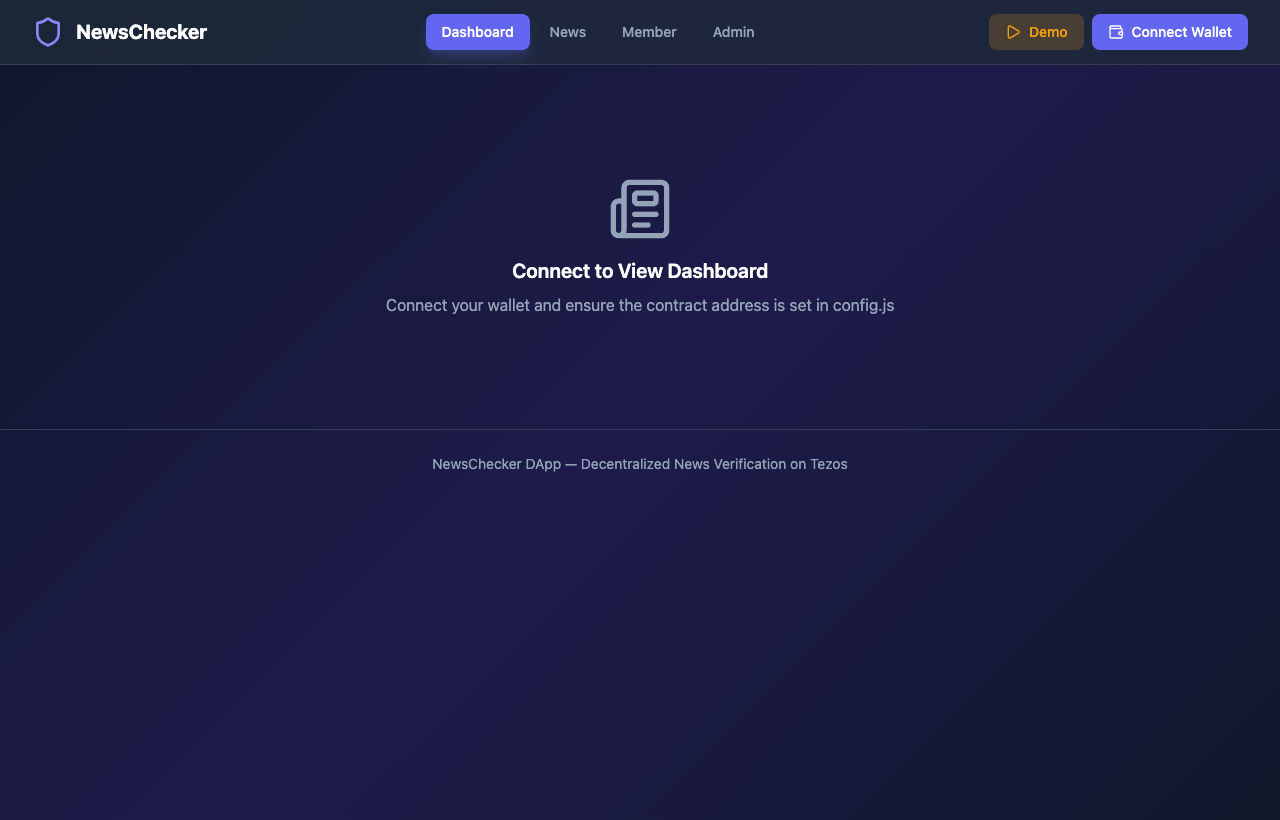
\includegraphics[width=0.82\textwidth]{screenshots/screen_landing.png}
}{%
  \fbox{\parbox{0.82\textwidth}{\centering\vspace{3.5cm}
    [Capture : Page d'accueil --- non connecté]\vspace{3.5cm}}}
}
\caption{Page d'accueil --- Avant connexion du portefeuille. Les boutons \emph{Demo} et \emph{Connect Wallet} sont visibles dans la barre de navigation.}
\label{fig:landing}
\end{figure}

\subsection{Dashboard}

\begin{figure}[H]
\centering
\begin{subfigure}[t]{0.48\textwidth}
\IfFileExists{screenshots/screen_dashboard_top.png}{%
  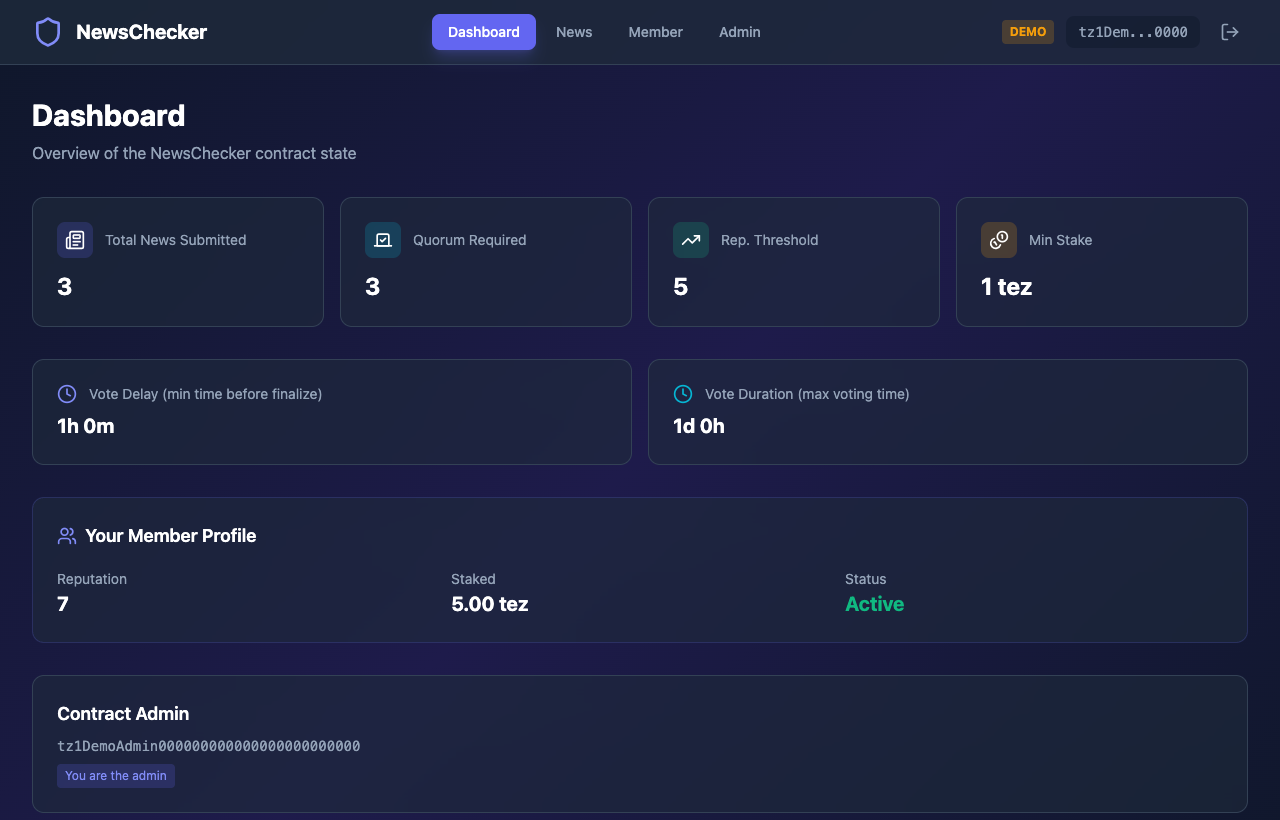
\includegraphics[width=\textwidth]{screenshots/screen_dashboard_top.png}
}{\fbox{\parbox{\textwidth}{\centering\vspace{3cm}[Dashboard haut]\vspace{3cm}}}}
\caption{Statistiques : Total News=3, Quorum=3, Rep. Threshold=5, Min Stake=1 tez}
\end{subfigure}
\hfill
\begin{subfigure}[t]{0.48\textwidth}
\IfFileExists{screenshots/screen_dashboard_bottom.png}{%
  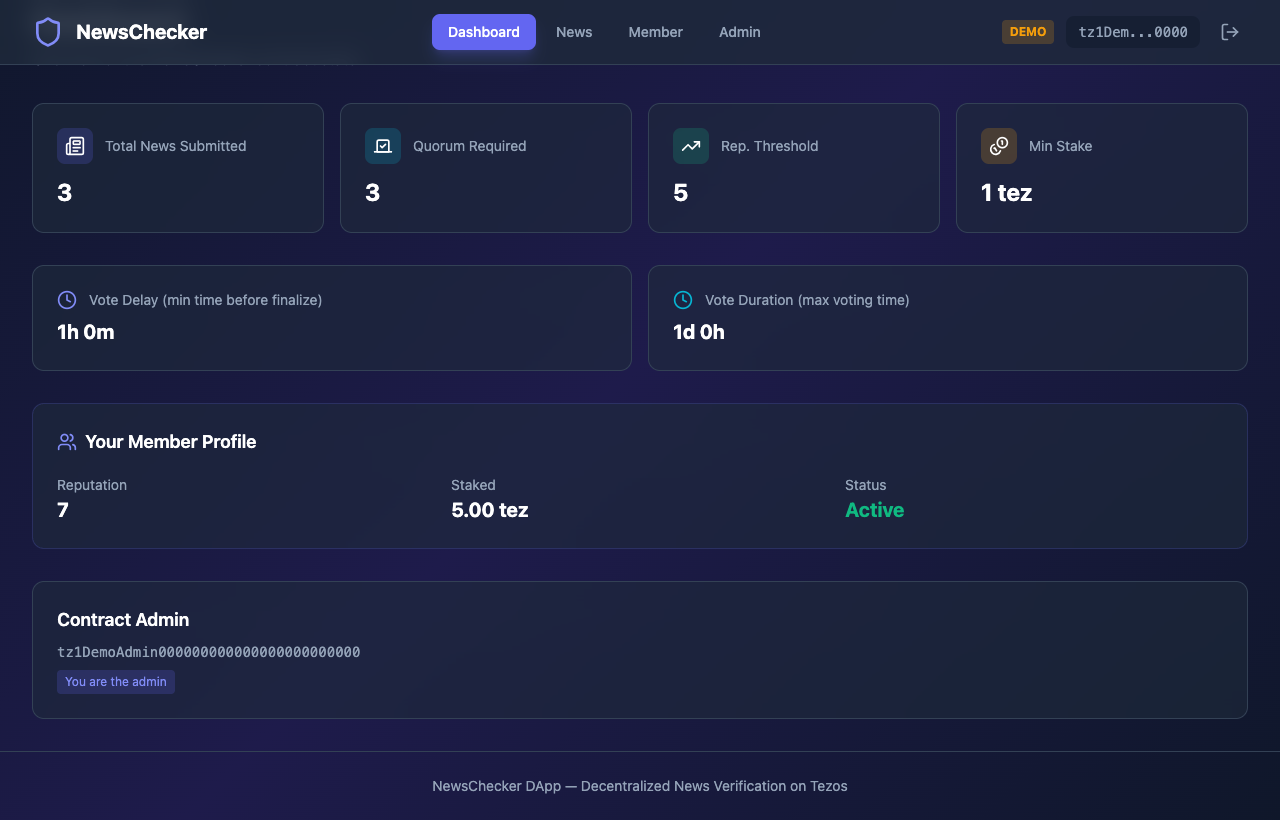
\includegraphics[width=\textwidth]{screenshots/screen_dashboard_bottom.png}
}{\fbox{\parbox{\textwidth}{\centering\vspace{3cm}[Dashboard bas]\vspace{3cm}}}}
\caption{Délais, profil membre (rep=7, stake=5 tez, Active), adresse admin}
\end{subfigure}
\caption{Dashboard --- Vue d'ensemble de l'état du contrat (mode démo)}
\label{fig:dashboard}
\end{figure}

\begin{infobox}[Métriques affichées sur le Dashboard]
\begin{itemize}
  \item \textbf{Total News Submitted :} 3 articles en mode démo (Voting, Fake, Real)
  \item \textbf{Quorum Required :} 3 votes minimum pour déclencher le Mode A
  \item \textbf{Rep. Threshold :} 5 --- seuil pour devenir Voter Confirmé
  \item \textbf{Min Stake :} 1 tez --- mise économique minimale
  \item \textbf{Vote Delay :} 1h 0m --- délai avant finalisation Mode A
  \item \textbf{Vote Duration :} 1j 0h --- durée maximale du vote
\end{itemize}
\end{infobox}

\subsection{Panneau News}

\begin{figure}[H]
\centering
\begin{subfigure}[t]{0.48\textwidth}
\IfFileExists{screenshots/screen_news_form.png}{%
  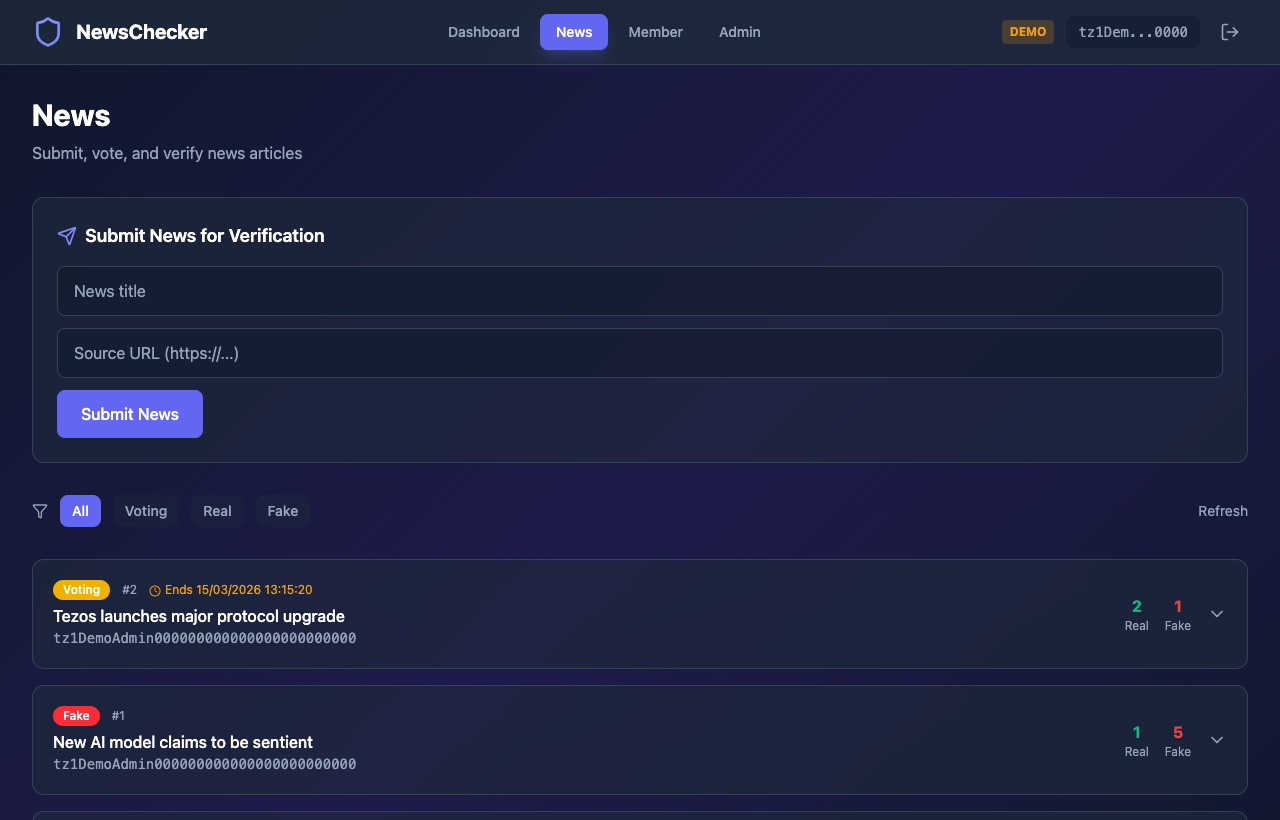
\includegraphics[width=\textwidth]{screenshots/screen_news_form.png}
}{\fbox{\parbox{\textwidth}{\centering\vspace{3cm}[News form]\vspace{3cm}}}}
\caption{Formulaire de soumission d'un article (titre + URL)}
\end{subfigure}
\hfill
\begin{subfigure}[t]{0.48\textwidth}
\IfFileExists{screenshots/screen_news_list.png}{%
  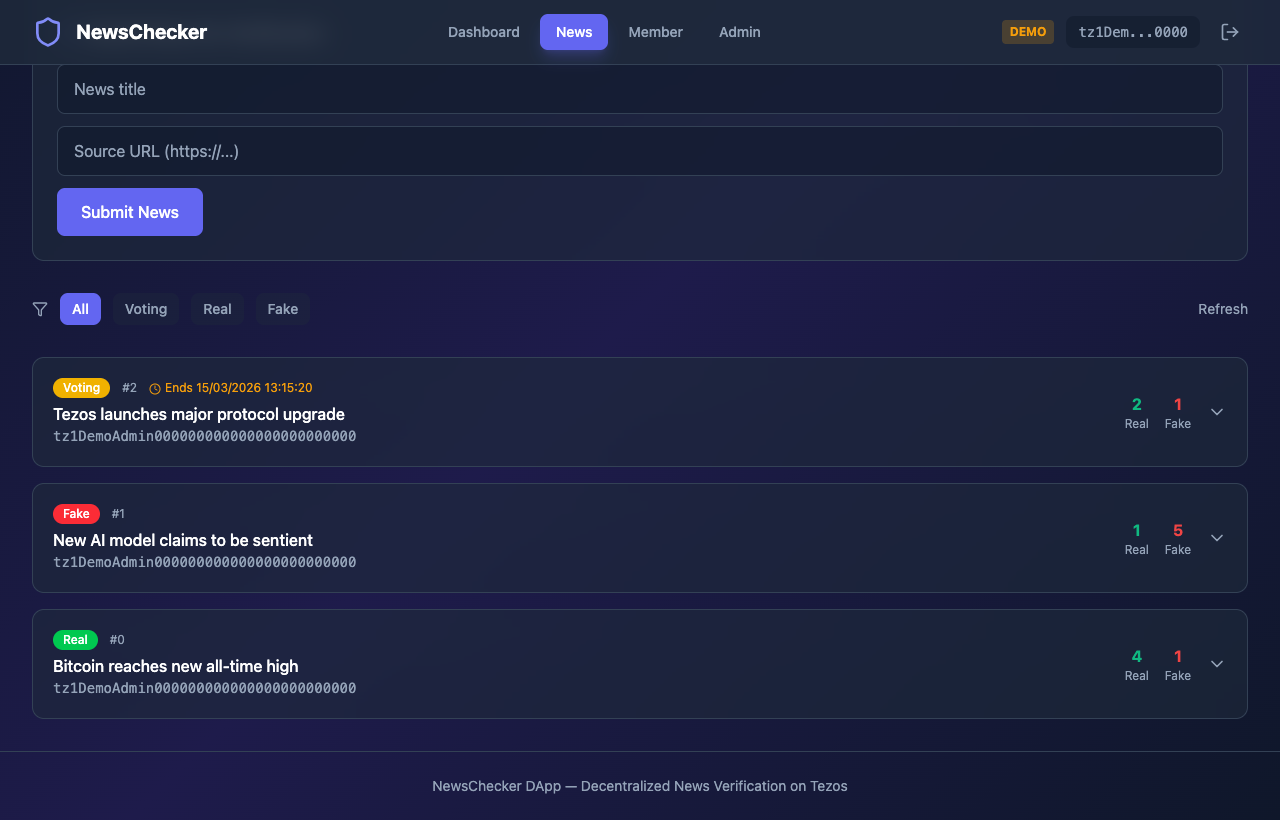
\includegraphics[width=\textwidth]{screenshots/screen_news_list.png}
}{\fbox{\parbox{\textwidth}{\centering\vspace{3cm}[News list]\vspace{3cm}}}}
\caption{Liste des articles avec badges de statut colorés}
\end{subfigure}
\caption{Panneau News --- Soumission et consultation des articles}
\label{fig:news}
\end{figure}

Les trois articles démo illustrent les statuts possibles :
\begin{itemize}
  \item \status{warning}{\#2 Voting} --- ``Tezos launches major protocol upgrade'' (2 REAL / 1 FAKE)
  \item \status{danger}{\#1 Fake}   --- ``New AI model claims to be sentient'' (1 REAL / 5 FAKE)
  \item \status{success}{\#0 Real}  --- ``Bitcoin reaches new all-time high'' (4 REAL / 1 FAKE)
\end{itemize}

\subsection{Panneau Membre}

\begin{figure}[H]
\centering
\begin{subfigure}[t]{0.48\textwidth}
\IfFileExists{screenshots/screen_member_top.png}{%
  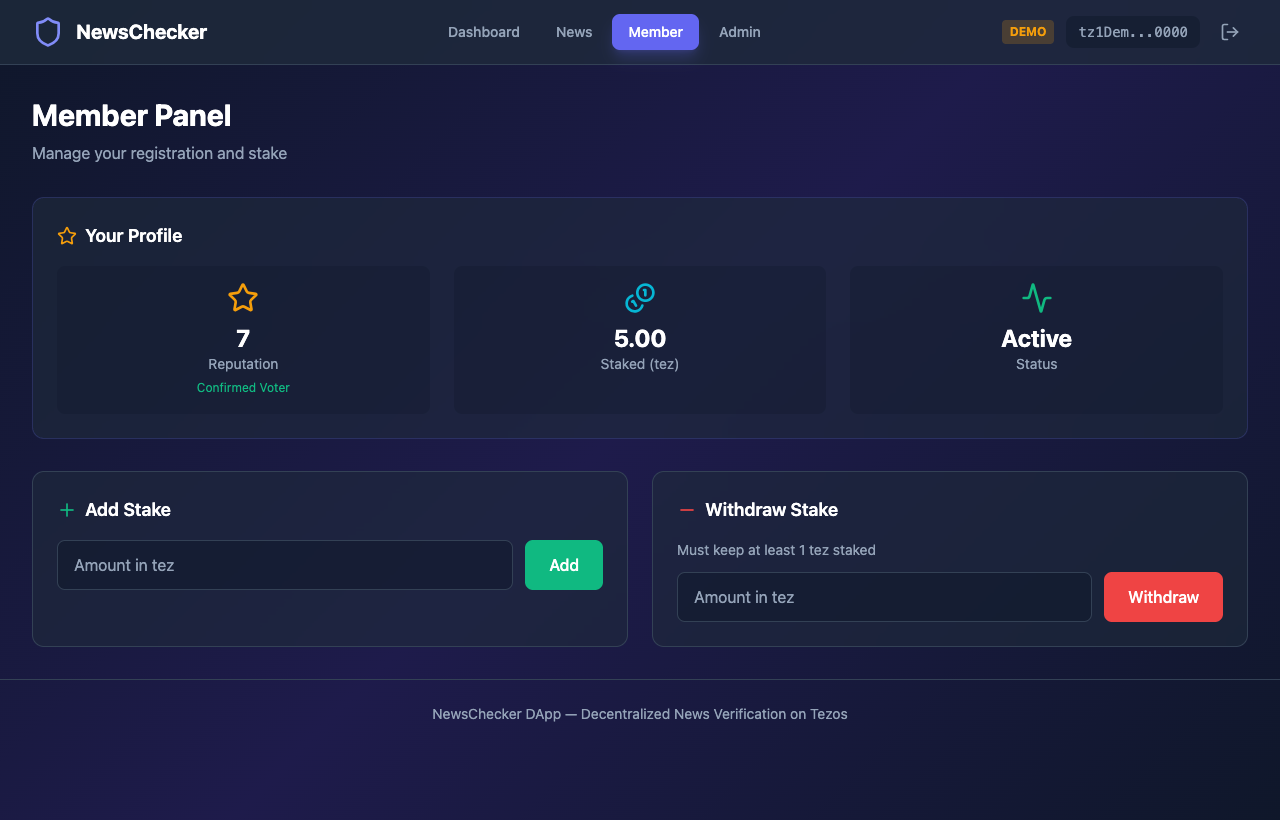
\includegraphics[width=\textwidth]{screenshots/screen_member_top.png}
}{\fbox{\parbox{\textwidth}{\centering\vspace{3cm}[Member top]\vspace{3cm}}}}
\caption{Profil : Réputation 7 (Confirmé), Stake 5.00 tez, Status Active}
\end{subfigure}
\hfill
\begin{subfigure}[t]{0.48\textwidth}
\IfFileExists{screenshots/screen_member_bottom.png}{%
  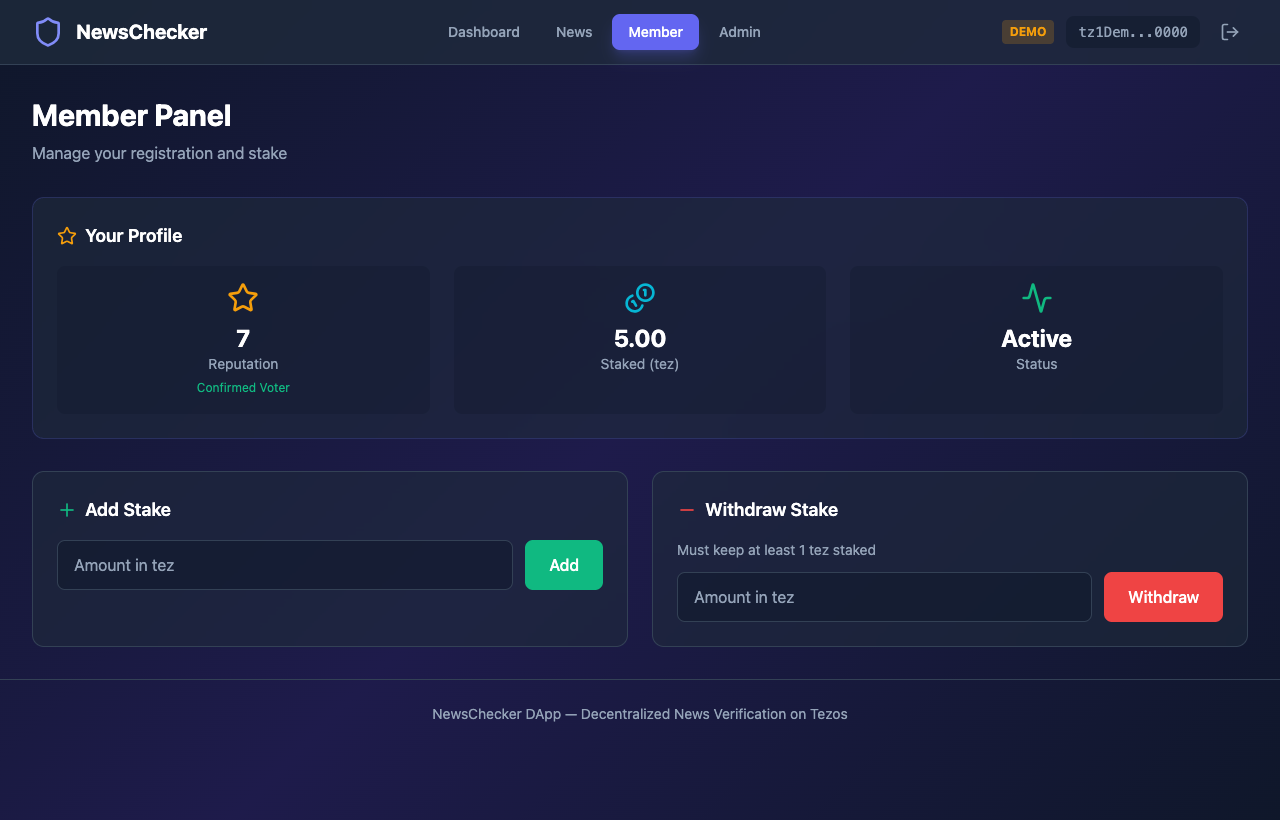
\includegraphics[width=\textwidth]{screenshots/screen_member_bottom.png}
}{\fbox{\parbox{\textwidth}{\centering\vspace{3cm}[Member bottom]\vspace{3cm}}}}
\caption{Formulaires Add Stake et Withdraw Stake}
\end{subfigure}
\caption{Panneau Membre --- Gestion de l'inscription et du stake}
\label{fig:member}
\end{figure}

\subsection{Panneau Admin}

\begin{figure}[H]
\centering
\begin{subfigure}[t]{0.48\textwidth}
\IfFileExists{screenshots/screen_admin_top.png}{%
  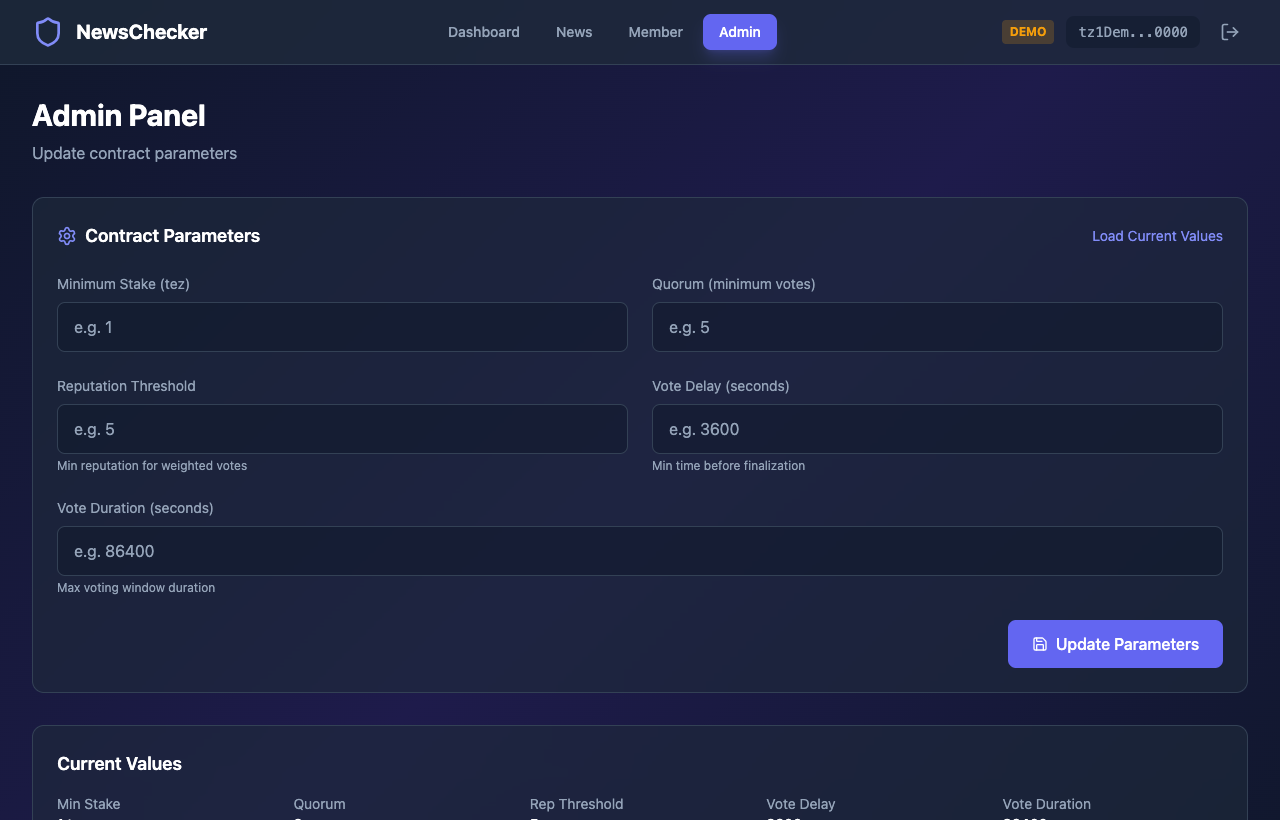
\includegraphics[width=\textwidth]{screenshots/screen_admin_top.png}
}{\fbox{\parbox{\textwidth}{\centering\vspace{3cm}[Admin top]\vspace{3cm}}}}
\caption{Paramètres du contrat : Min Stake, Quorum, Rep Threshold}
\end{subfigure}
\hfill
\begin{subfigure}[t]{0.48\textwidth}
\IfFileExists{screenshots/screen_admin_bottom.png}{%
  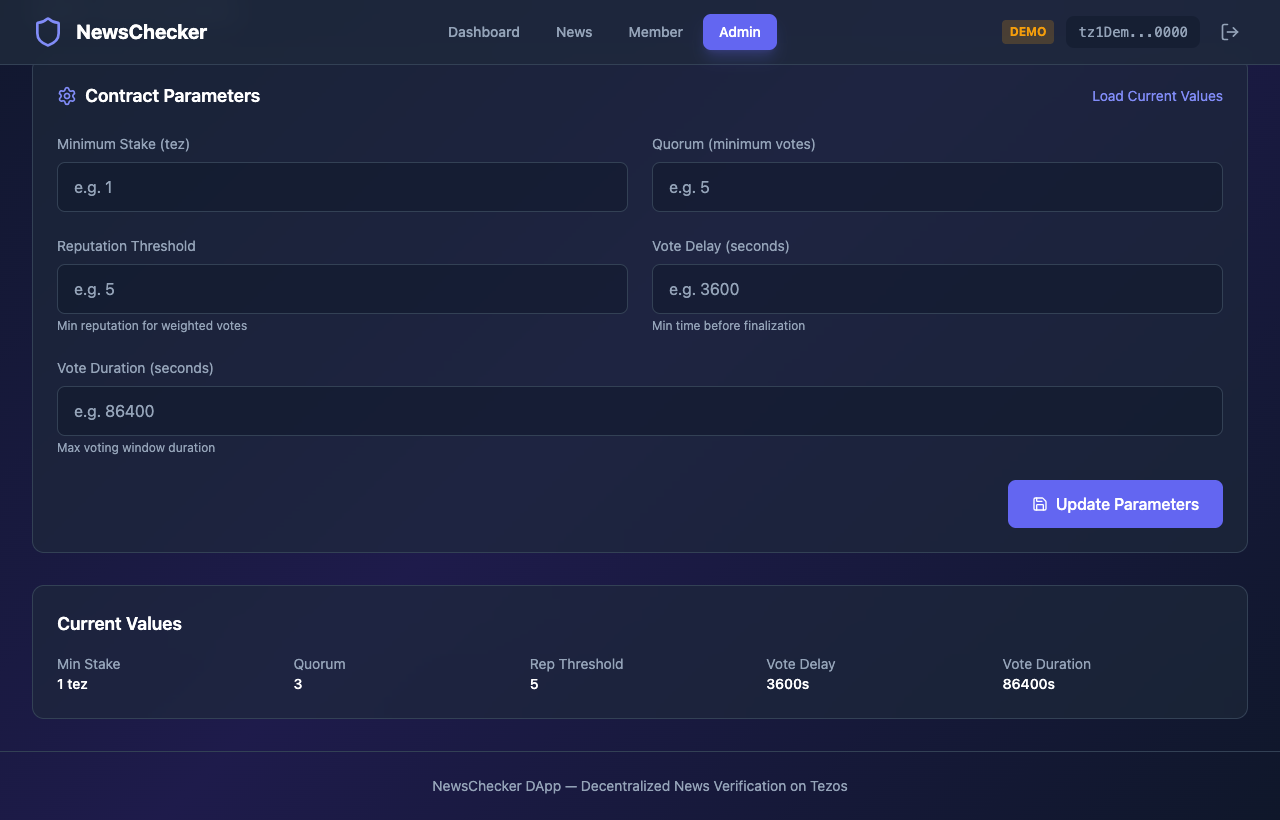
\includegraphics[width=\textwidth]{screenshots/screen_admin_bottom.png}
}{\fbox{\parbox{\textwidth}{\centering\vspace{3cm}[Admin bottom]\vspace{3cm}}}}
\caption{Vote Delay, Vote Duration, bouton Update Parameters}
\end{subfigure}
\caption{Panneau Admin --- Mise à jour des paramètres (admin uniquement)}
\label{fig:admin}
\end{figure}

%% ════════════════════════════════════════════════════════════
\section{Scénarios de Test}
%% ════════════════════════════════════════════════════════════

\subsection{Suite de tests SmartPy}

\begin{longtable}{L{4.2cm} L{3.8cm} L{5cm}}
\toprule
\rowcolor{primary!15}
\textbf{Nom du test} & \textbf{Mode testé} & \textbf{Résultat attendu} \\
\midrule
\endhead

\texttt{test\_finalize\_after\_delay}
  & Mode A (quorum + délai)
  & Finalise après 3700s avec quorum=3 $\checkmark$ \\
\rowcolor{lightgray}
\texttt{test\_finalize\_after\_deadline}
  & Mode B (timeout)
  & Finalise après 90000s même sans quorum $\checkmark$ \\

\texttt{test\_vote\_after\_deadline\_blocked}
  & Deadline vote
  & Vote refusé après 86400s $\checkmark$ \\
\rowcolor{lightgray}
\texttt{test\_no\_votes\_cannot\_finalize}
  & Aucun vote
  & \texttt{NO\_VOTES} même après deadline $\checkmark$ \\

\texttt{test\_reputation\_growth}
  & Progression rep.
  & rep $1 \to 3 \to 5 \to 7$ en 3 tours $\checkmark$ \\
\rowcolor{lightgray}
\texttt{test\_sybil\_attack}
  & Anti-Sybil
  & 5 attaquants (poids=0) vs 2 confirmés $\to$ FAKE $\checkmark$ \\

\texttt{test\_bad\_voter\_falls}
  & Pénalité rep.
  & rep $5 \to 2$ après vote incorrect $\checkmark$ \\
\rowcolor{lightgray}
\texttt{test\_double\_vote}
  & Vote double
  & \texttt{ALREADY\_VOTED} bloqué $\checkmark$ \\

\texttt{test\_admin\_and\_staking}
  & Admin + staking
  & Params mis à jour, non-admin bloqué $\checkmark$ \\
\bottomrule
\caption{Suite complète des 9 tests SmartPy}
\end{longtable}

\subsection{Codes d'erreur}

\begin{table}[H]
\centering
\renewcommand{\arraystretch}{1.4}
\begin{tabular}{L{4.5cm} L{4.5cm} L{3.5cm}}
\toprule
\rowcolor{primary!15}
\textbf{Condition} & \textbf{Code d'erreur} & \textbf{Entrypoint} \\
\midrule
Déjà inscrit              & \texttt{ALREADY\_REGISTERED}  & \texttt{register} \\
\rowcolor{lightgray}
Mise insuffisante          & \texttt{INSUFFICIENT\_STAKE}   & \texttt{register} \\
Non inscrit                & \texttt{NOT\_REGISTERED}       & Tous \\
\rowcolor{lightgray}
News inexistante           & \texttt{NEWS\_NOT\_FOUND}      & \texttt{vote}, \texttt{finalize} \\
Statut incorrect           & \texttt{NOT\_IN\_VOTING}       & \texttt{vote}, \texttt{finalize} \\
\rowcolor{lightgray}
Deadline dépassée          & \texttt{VOTING\_ENDED}         & \texttt{vote} \\
Déjà voté                  & \texttt{ALREADY\_VOTED}        & \texttt{vote} \\
\rowcolor{lightgray}
Finalisation impossible    & \texttt{CANNOT\_FINALIZE\_YET} & \texttt{finalize} \\
Aucun vote                 & \texttt{NO\_VOTES}             & \texttt{finalize} \\
\rowcolor{lightgray}
Solde insuffisant          & \texttt{NOT\_ENOUGH}           & \texttt{withdraw\_stake} \\
Sous le minimum            & \texttt{BELOW\_MINIMUM}        & \texttt{withdraw\_stake} \\
\rowcolor{lightgray}
Non administrateur         & \texttt{NOT\_ADMIN}            & \texttt{update\_params} \\
\bottomrule
\end{tabular}
\caption{Codes d'erreur du contrat (12 conditions)}
\end{table}

%% ════════════════════════════════════════════════════════════
\section{Analyse de Sécurité}
%% ════════════════════════════════════════════════════════════

\subsection{Vecteurs d'attaque et défenses}

\begin{table}[H]
\centering
\renewcommand{\arraystretch}{1.5}
\begin{tabular}{L{3.5cm} L{4.5cm} C{2.5cm}}
\toprule
\rowcolor{primary!15}
\textbf{Attaque} & \textbf{Mécanisme de défense} & \textbf{Efficacité} \\
\midrule
\textbf{Sybil (multi-comptes)} & Poids=0 en probatoire jusqu'à rep$\geq$5 & Très élevée \\
\rowcolor{lightgray}
\textbf{Vote précipité}        & Mode A : délai min obligatoire            & Élevée \\
\textbf{Collusion (inactifs)}  & Mode B : finalisation après deadline      & Élevée \\
\rowcolor{lightgray}
\textbf{Manipulation admin}    & Admin limité à update\_params uniquement  & Bonne \\
\textbf{Vote sans enjeu}       & Staking minimum obligatoire               & Élevée \\
\rowcolor{lightgray}
\textbf{Double vote}           & Clé \texttt{(news\_id, address)} unique   & Totale \\
\bottomrule
\end{tabular}
\caption{Analyse des vecteurs d'attaque et contre-mesures}
\end{table}

\subsection{Progression de réputation}

\begin{figure}[H]
\centering
\begin{tikzpicture}
\begin{axis}[
  xlabel={Nombre de votes corrects consécutifs},
  ylabel={Réputation},
  xmin=0, xmax=10,
  ymin=0, ymax=22,
  xtick={0,1,...,10},
  ytick={0,2,4,5,6,8,10,12,14,16,18,20},
  grid=major,
  grid style={dashed, gray!30},
  legend pos=north west,
  width=13cm, height=7cm,
  title={\textbf{Évolution de la réputation par votes corrects}}
]
\addplot[color=primary, mark=*, line width=2pt, mark size=3pt]
  coordinates {(0,1)(1,3)(2,5)(3,7)(4,9)(5,11)(6,13)(7,15)(8,17)(9,19)(10,21)};
\addlegendentry{Progression nominale}

\addplot[color=success, dashed, line width=1.5pt]
  coordinates {(0,5)(10,5)};
\addlegendentry{Seuil Confirmé (rep=5)}

\addplot[color=warning, dotted, line width=1.5pt]
  coordinates {(0,1)(10,1)};
\addlegendentry{Réputation initiale}
\end{axis}
\end{tikzpicture}
\caption{Progression de la réputation sur 10 votes corrects consécutifs}
\label{fig:repchart}
\end{figure}

%% ════════════════════════════════════════════════════════════
\section{Guide de Déploiement}
%% ════════════════════════════════════════════════════════════

\subsection{Déploiement du contrat sur Ghostnet}

\begin{enumerate}
  \item \textbf{Obtenir des tez de test} via le faucet Ghostnet :\\
    \url{https://faucet.ghostnet.teztnets.com/}

  \item \textbf{Compiler et déployer} via SmartPy IDE :\\
    \url{https://smartpy.io/ide}
    \begin{itemize}
      \item Coller le code du contrat dans l'éditeur
      \item Cliquer \textbf{Run} puis naviguer vers \textbf{Deploy}
      \item Sélectionner le réseau \textbf{Ghostnet}
      \item Connecter Temple ou Kukai Wallet
      \item Confirmer la transaction (coût : environ 1 tez)
    \end{itemize}

  \item \textbf{Récupérer l'adresse} \texttt{KT1...} du contrat déployé via\\
    \url{https://ghostnet.tzkt.io}

  \item \textbf{Configurer le frontend} dans \texttt{src/config.js} :
\end{enumerate}

\begin{lstlisting}[language=JSX, caption={Configuration src/config.js}]
export const CONTRACT_ADDRESS = 'KT1VotreAdresseContratIci...';
export const RPC_URL          = 'https://ghostnet.tezos.marigold.dev';
export const NETWORK          = 'ghostnet';
\end{lstlisting}

\subsection{Lancement du frontend}

\begin{lstlisting}[language=bash, caption={Commandes de démarrage}]
# Installer les dependances
npm install

# Lancer en developpement (http://localhost:5173)
npm run dev

# Build de production
npm run build

# Preview du build de production
npm run preview
\end{lstlisting}

\begin{warnbox}[Wallet requis pour le mode réel]
Pour interagir avec le contrat déployé, les utilisateurs ont besoin d'un portefeuille Tezos compatible Beacon :
\begin{itemize}
  \item \textbf{Temple Wallet :} \url{https://templewallet.com} (recommandé pour Ghostnet)
  \item \textbf{Kukai :} \url{https://kukai.app}
\end{itemize}
En attendant le déploiement, le \textbf{Mode Démo} permet de tester toutes les fonctionnalités sans portefeuille.
\end{warnbox}

%% ════════════════════════════════════════════════════════════
\section{Conclusion}
%% ════════════════════════════════════════════════════════════

NewsChecker démontre la faisabilité d'un système de vérification des nouvelles décentralisé, transparent et résistant aux manipulations. Les principaux apports du projet sont :

\begin{successbox}[Résultats obtenus]
\begin{itemize}
  \item \textbf{Contrat fonctionnel :} 7 entrypoints, 12 codes d'erreur, 9 tests automatisés validés
  \item \textbf{Résistance Sybil prouvée :} Le vote pondéré par réputation neutralise les comptes fantômes
  \item \textbf{Double mode de finalisation :} Garantit la résolution même en cas de faible participation
  \item \textbf{Interface complète :} Mode Démo intégré pour tester sans déploiement réel
  \item \textbf{Gouvernance paramétrable :} L'admin peut ajuster le comportement sans redéploiement
\end{itemize}
\end{successbox}

\subsection{Perspectives d'amélioration}

\begin{itemize}
  \item \textbf{Pénalité de stake :} Déduire une partie du stake des mauvais voteurs
  \item \textbf{Catégorisation :} Organiser les articles par thématiques (politique, science, sport)
  \item \textbf{Mécanisme d'appel :} Permettre le recours après finalisation
  \item \textbf{DAO Governance :} Remplacer l'admin unique par un vote collectif des membres confirmés
  \item \textbf{Oracle externe :} Intégrer des sources tierces de fact-checking
  \item \textbf{Mainnet :} Migration vers le réseau principal Tezos
\end{itemize}

\vspace{1.5cm}
\begin{center}
\begin{tikzpicture}
  \node[draw=primary, fill=primary!8, rounded corners=7pt,
        inner sep=14pt, line width=1.5pt]{
    \begin{minipage}{11cm}
      \centering
      {\large\bfseries\color{darkbg} NewsChecker DApp}\\[6pt]
      {\small\color{mutedtext}
        Smart Contract SmartPy \textbullet{} Tezos Ghostnet \textbullet{}
        React 19 \textbullet{} Taquito 20 \textbullet{} Beacon SDK 4}\\[6pt]
      {\small\color{primary}
        \url{https://github.com/votre-repo/news-checker-dapp}}
    \end{minipage}
  };
\end{tikzpicture}
\end{center}

\end{document}
